\documentclass[./main.tex]{subfiles}

\begin{document}
\section{Autoencoders, Stacked Hourglass, PCA and $K$-Means}\label{sec:algorithms}
In this section the various algorithms and architectures used throughout this thesis is described and explained in details. The section starts off with Section \ref{subsec:AE}, where we will be giving a brief introduction to autoencoders. Throughout Section \ref{subsec:SHG} the Stacked hourglass, used for pose estimation, is described. Then, in Section \ref{subsec:PCA} the algorithm of Principal Components Analysis is described. In the last section, Section \ref{subsec:K_means}, $K$-Means clustering is described.

\subsection{Autoencoders}\label{subsec:AE}
\begin{figure}[htbp]
    \centering
    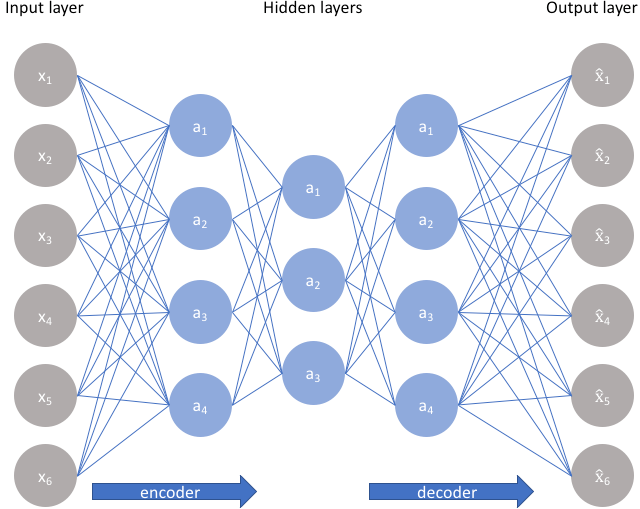
\includegraphics[width = 7 cm]{entities/AE.png}
    \caption{Visualization of an undercomplete autoencoder \cite{AE}}
    \label{fig:AE}
\end{figure}
\noindent \textit{Autoencoders} is a class of neural networks that are trained to output the input of the model. An autoencoder consists of two parts: the \textit{encoder} and the \textit{decoder}, where each part usually consist of multiple hidden layers. When data is fed to the autoencoder, the data is passed through the encoder, which then passes the data to the decoder, where the data is again processed and finally returned \cite{DeepLearning}. 
\\
\\
If all of the layers of the autoencoder have the same dimensionality, the network can easily learn how to copy the input to its output. For this reason we often talk about \textit{undercomplete} autoencoders instead, where the dimension of the output of the encoder is smaller than the dimension of the input and output of the network, as visualized in Figure \ref{fig:AE}. By making use of an undercomplete autoencoder, the encoder learns how to encode the input to a lower dimensionality, forcing the network to learn the most important features of the training data \cite{DeepLearning}.
\\
\\
To make the autoencoder more robust in relation to small variances, some noise is usually added to the input of the data during training. The noisy training data is then passed through the network and compared to the non-noisy training data, when the loss is computed \cite{DeepLearning}.

\subsection{Stacked Hourglass}\label{subsec:SHG}
When performing the pose estimation in section \ref{experiement}, we will be implementing and using the \textit{Stacked hourglass} described by Newell \textit{et al.} \cite{Newell}. The following description and explanation of the architecture is based on an interpretation of Newell \textit{et al.} \cite{Newell} and Camilla Olsen \cite{Camilla}.

\subsubsection{Motivation behind using the Stacked Hourglass}\label{subsec:reasoning}
We have decided to make use of the Stacked hourglass described by Newell \textit{et al.}, as it is an architecture that has shown state-of-the-art results. At the same time the architecture of the network is similar to the architecture of autoencoders, making the architecture useful for encoding the data into a lower dimension, which can be useful in section \ref{sec:XAI}, when we will be doing the interpretation of the model.

\subsubsection{The Residual Module}
\begin{figure}[htbp]
    \centering
    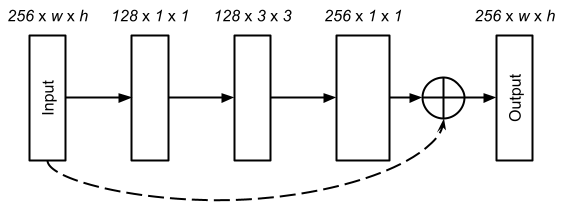
\includegraphics[height = 2 cm]{entities/Residual.png}
    \caption{Visualization of the residual module \cite{Newell}}
    \label{fig:residual}
\end{figure}
\noindent The Stacked hourglass makes heavily use of so-called \textit{residual modules}, one of which is visualized in Figure \ref{fig:residual}. The module works by taking an input, which is sent through a $1 \times 1$ and a $3 \times 3$ convolution, each with $128$ channels. Then, the $128$ output featuremaps are sent through a $1 \times 1$ convolution with $256$ channels. Lastly, element-wise addition is then used to add the $256$ output featuremaps to the input of the module, which the module then returns. All convolutions are followed by an acitvation function and are \textit{same convolutions}, meaning the output featuremaps are of the same dimensions as the input featuremeaps.

\subsubsection{The Hourglass}
\begin{figure}[htbp]
    \centering
    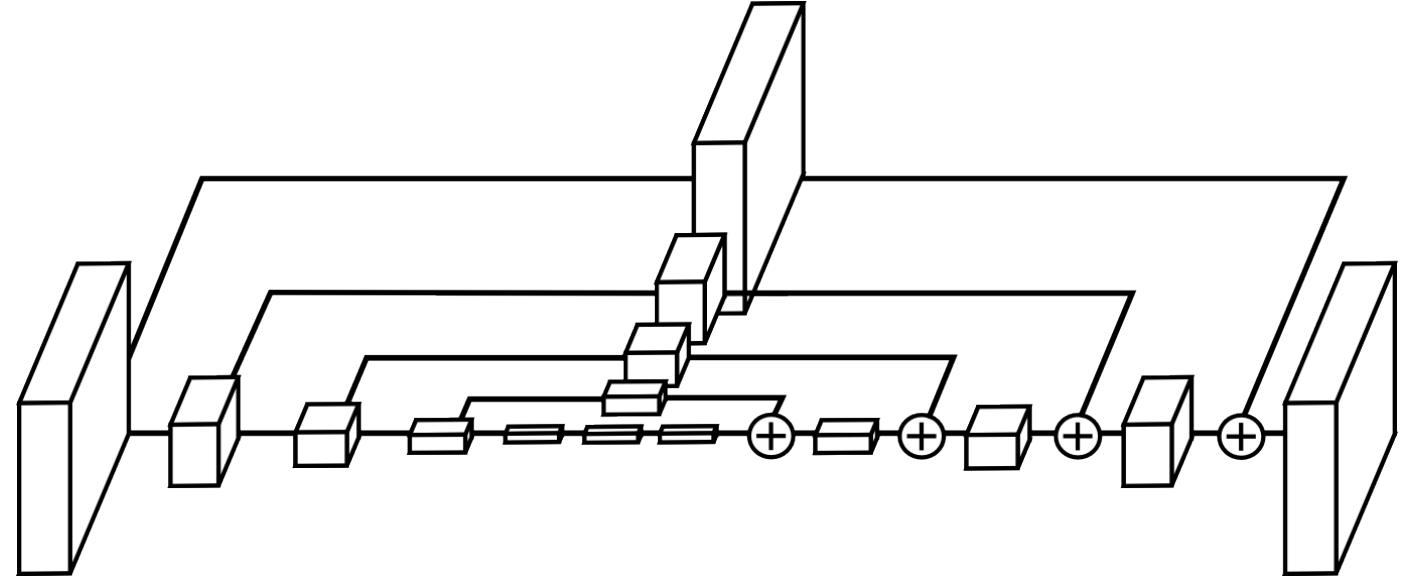
\includegraphics[height = 4 cm]{entities/Hourglass.png}
    \caption{Visualization of a single hourglass \cite{Newell}}
    \label{fig:hourglass}
\end{figure}
\noindent The Stacked hourglass consists of hourglasses, where each hourglass is split into an encoder, where the featuremaps is downsampeld, and a decoder, where the featuremaps are upsampled. The hourglass is symmetric, in the sense, that it has an equal amount of downsampling layers in the encoder as there are upsampling layers in the decoder. In Figure \ref{fig:hourglass} a single hourglass han been visualized, where each box is a residual module.
\\
\\
The hourglass works by using residuals and max poolings to process features down to a low resolution. Then, nearest neighbor upsampling is used to upsample the featuremaps until the featuremaps have the same dimensions as the input of the hourglass. Before each max pool in the encoder, the network branches off and applies a residual. The output of this residual is then added back element-wise to the corresponding level in the decoder, which helps to ensure that lost information from the encoder is kept. This is then fed into a residual in the decoder.
\\
\\
Between the encoder and decoder the network has a bottleneck, where no downsampling or upsampling happens, instead only residuals are processing the featuremaps. After the decoder two $1 \times 1$ convolution layers er applied to produce the final predictions of the network.

\subsubsection{The Stacked Hourglass}
\begin{figure}[htbp]
    \centering
    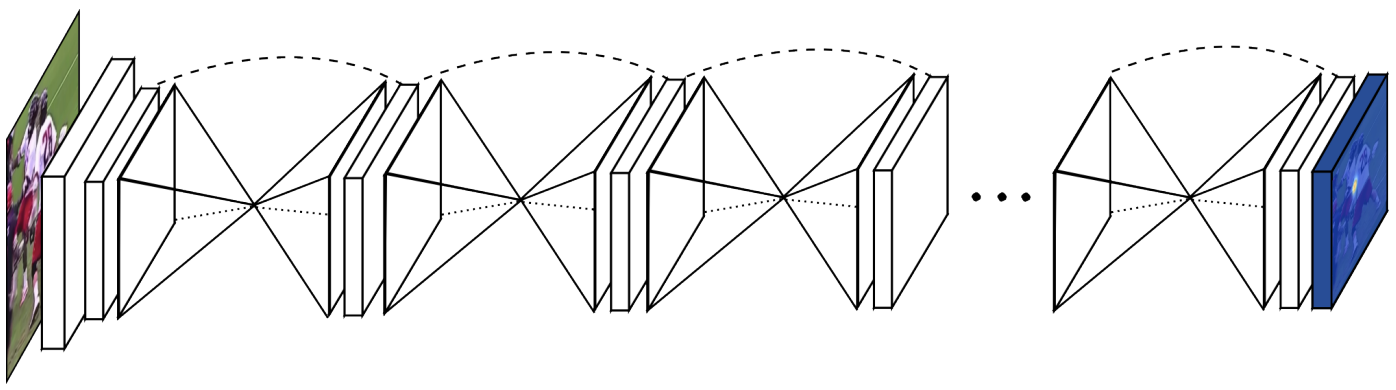
\includegraphics[height = 4 cm]{entities/SHG.png}
    \caption{Visualization of the Stacked hourglass \cite{Newell}}
    \label{fig:SHG}
\end{figure}
\noindent The full network is build by stacking multiple hourglasses end-to-end, making the output of one hourglass be the input of the next hourglass, as shown in Figure \ref{fig:SHG}, which makes each hourglass reevaluate estimates. To evaluate each hourglass, intermediate supervision is used by applying a loss to each hourglass' intermediate prediction.
\\
\\
The input of the network is a $256 \times 256$ RGB-image. To lower the memory usage, the network starts off with a $7 \times 7$ convolution layer with stride 2, followed by a residual module and max pooling to bring the resolution down to $64 \times 64$, which is then input to the first hourglass.
\\
\\
By the end the whole network outputs $n$ heatmaps corresponding to the $n$ joints it should predict for a single person. The prediction of a joint is thus the maximum activation of the corresponding heatmap.

\subsection{Principal Components Analysis (PCA)}\label{subsec:PCA}
\begin{algorithm}[htbp]
    \caption{PCA \cite{MAD_book}}
    \begin{algorithmic}[1]
        \Require Input data $\bm{Y} \in \mathbb{R}^{N \times D}$, with feature columns $\bm{y}_1, ..., \bm{y}_N$.
        \Require Wanted output dimensions $k$
        \State Let each feature column have zero mean by subtracting the corresponding mean, $\bar{y} = \frac{1}{N} \sum_{n = 1} ^N \bm{y}_n$, from each feature column
        \State Compute the sample covariance matrix $\bm{C} = \frac{1}{N} \sum_{n = 1} ^N \bm{y}_n \bm{y}_n ^T$ 
        \State Find the $D$ eigenvector/eigenvalue pairs of the covariance matrix
        \State Find the eigenvectors, $\bm{w}_1, ..., \bm{w}_k \in \mathbb{R}^D$, corresponding to the $k$ highest eigenvalues
        \State Let $\bm{W} = \left[ \bm{w}_1, ..., \bm{w}_k \right]$, that is, the $D \times k$ matrix created by placing the $k$ eigenvectors alongside one another
        \State Let $\bm{X} = \bm{Y} \bm{W}$ be the projection of $Y$ down to $k$ dimensions
        \State \textbf{return} $\bm{X}$
    \end{algorithmic}
    \label{Algorithm:PCA}
\end{algorithm}
\noindent It is very common, that a given dataset has an enormous amount of dimensions. This is quickly become a problem, as it can be difficult to visualize or it can lead to other problems, such as models becoming too complex, thus being prone to overfitting. This is a common phenomen called the \textit{Curse of Dimensionality} \cite{ESL}. For this reason multiple techniques have been developed for reducing the dimensions of a given dataset. We have already seen in Section \ref{subsec:AE}, how autoencoders can be used as non-linear dimensionality reduction. Another very common technique for reducing the dimension of a dataset is \textit{Principal Components Analysis} (\textit{PCA}).
\\
\\
PCA is an unsupervised linear projection method used for reducing the dimension of a dataset from $D$ down to $k$ dimensions. The algorithm works by finding the $k$ orthogonal vectors that maximizes the variance of the input data. \cite{MAD_book} 
\\
\\
The pseudocode of the algorithm has been visualized in Algorithm \ref{Algorithm:PCA}. The algorithm starts off by finding the sample covariance matrix $\bm{C}$. It then finds the $k$ vectors, that maximizes the variance of the input data. The $k$ vectors that maximizes the variance are the $k$ eigenvectors with the corresponding highest eigenvalues. Thus, the projection with the first eigenvector captures the most variance, the projection with the second eigenvector captures the second most variance, and so on. The projection down to $k$ dimensions then happens by stacking the $k$ eigenvectors, forming a $D \times k$ matrix, where $D$ is the input dimensions, which is then multiplied with the input data, resulting in the projected data. \cite{MAD_book}

\subsection{$K$-Means Clustering}\label{subsec:K_means}
Often we want to find patterns in data that has not been labelled. One common group of techniques for this purpose is the \textit{clustering algorithms}, that are used to group observations into clusters, such that observations from the same cluster are more similar, than observations from different clusters. One common clustering technique is $K$\textit{-Means}.
\\
\\
$K$-Means is a unsupervised method used for clustering observations into $K$ groups of similar observations, such that no observation occurs in multiple clusters. The algorithm uses distance as a measure of similarity, such that observations closer to each other are more likely to being grouped to the same cluster, than two observations far appart. In the middle of each cluster is a synthetic observation (that is, not a real observation), called the \textit{centroid}, which is defined as the mean of the cluster. The pseudocode of the algorithm has been visualized in Algorithm \ref{Algorithm:KMeans}. The algorithm is an iterative process, which works firstly by assigning each observation to the closest centroid. Next, each centroid is updated accordingly. This is done until the assigning of each observation is unchanged \cite{MAD_book}.
\\
\\
$K$-Means is guaranteed to converge to a local minimum of the total distance between the objects and their corresponding centroid, however, it is not guaranteed to reach the global minimum. This only depends on the initial position of the centroids. To partly overcome this problem it is common to run the algorithm multiple times with different random initial positions of the centroids and use the best solution as the final output \cite{MAD_book}.

\begin{algorithm}[htbp]
    \caption{$K$-Means \cite{DS_manual}}
    \begin{algorithmic}[1]
        \Require Input data $\bm{X} \in \mathbb{R}^{n \times m}$
        \Require Amount of clusters $k$
        \State Select $k$ points as initial cluster centers $\bm{C}_1, ..., \bm{C}_k$
        \While{not converged}
            \For{$1 \leq 1 \leq n$}
                \State Map point $p_i$ to its nearest cluster center $\bm{C}_j$
            \EndFor

            \For{$1 \leq j \leq k$}
                \State Compute centroid $\bm{C}'_j$ of the points nearest $\bm{C}_j$
            \EndFor

            \For{$1 \leq j \leq k$}
                \State Set $\bm{C}_j = \bm{C}'_j$
            \EndFor
        \EndWhile
    \end{algorithmic}
    \label{Algorithm:KMeans}
\end{algorithm}


\end{document}